\documentclass{article}

\usepackage{a4}
\usepackage{amsmath}
\usepackage{amssymb}
\usepackage{ctex}
\usepackage{booktabs}
\usepackage{graphicx}
\usepackage{subfigure}
\usepackage{subcaption}
\usepackage{float}
\usepackage{hyperref}
\usepackage{xurl}
\usepackage{enumitem}
\usepackage{array}
\usepackage{longtable}
\usepackage{multirow}
\usepackage{fvextra}

\hypersetup{colorlinks=true,linkcolor=black,urlcolor=blue,citecolor=black}
\setlist[itemize]{nosep,leftmargin=1.8em}
\setlist[enumerate]{nosep,leftmargin=1.8em}
\captionsetup{font=small}
\setlength{\emergencystretch}{3em}
\renewcommand{\arraystretch}{1.2}
\RecustomVerbatimEnvironment{verbatim}{Verbatim}{
  breaklines=true,
  breakanywhere=true,
  fontsize=\small
}
\newcommand{\sourcecode}[2]{
  \subsubsection*{#1}
  \noindent 对应文件：\path{#2}
  \VerbatimInput[
    breaklines=true,
    breakanywhere=true,
    fontsize=\small
  ]{#2}
}

\title{计算机组成原理 Project1 实验报告（Week 2）\\8位定点卷积--激活--池化链运算器设计}
\author{鲁昕宁 2414015}
\date{2026年4月26日}

\begin{document}

\maketitle
\begin{center}
  \url{https://github.com/SidneyLu/Computer-Organization-and-Design-NKU-CS/tree/master/project1}
\end{center}

\newpage

\section{里程碑2：链式运算器集成与系统仿真}
\subsection{串行链式运算器实现}
本实验第一组实现了基于串行状态机的链式运算器，完整支持 ``卷积 $\rightarrow$ ReLU $\rightarrow$ 池化'' 三段链路。

\sourcecode{顶层 \texttt{cnn\_compare\_base\_top} 的 Verilog 源码}{../src/baseline/cnn_compare_base_top.v}
\sourcecode{模块 \texttt{cnn\_chain\_core\_base} 的 Verilog 源码}{../src/baseline/cnn_chain_core_base.v}

优化版本的链式运算器（BoothWallace、SIMD、流水线、DSP版本）源码与仿真结果详见第三部分。

\subsection{标准样例与手算结果}
系统 testbench \texttt{tb\_cnn\_core} 采用如下标准输入：
\begin{itemize}
  \item 图像矩阵为从 1 到 25 的顺序数列，按行优先排布为 $5\times 5$；
  \item 卷积核 9 个元素均为 1。
\end{itemize}

对应的卷积结果为：
\[
\begin{bmatrix}
63 & 72 & 81 \\
108 & 117 & 126 \\
153 & 162 & 171
\end{bmatrix}
\]
ReLU 后保持不变。继续执行 $2\times 2$ 平均池化，可得到：
\[
\begin{bmatrix}
90 & 99 \\
135 & 144
\end{bmatrix}
\]
在 \texttt{out\_flat\_u8x4} 中，该结果被打包为 \texttt{32'h9087635A}。

\subsection{基础模块系统仿真结果}
系统级仿真命令为：
\begin{verbatim}
powershell -ExecutionPolicy Bypass -File .\scripts\run_vivado_sim.ps1 -Mode system
\end{verbatim}

\texttt{tb\_cnn\_core} 对串行顶层拉起 \texttt{start}，并显式检查输出与延迟行为。结果如表 \ref{tab:sim-system-base} 所示。

\begin{table}[H]
\centering
\caption{基础模块系统仿真结果}
\label{tab:sim-system-base}
\begin{tabular}{lccc}
\toprule
实验组 & 输出结果 & 延迟周期 \\
\midrule
串行 &  \texttt{32'h9087635A} & 96 \\
\bottomrule
\end{tabular}
\end{table}

XSIM 日志中可以直接看到如下 PASS 信息：
\begin{verbatim}
CASE=1 PASS cycles=96 out=9087635a
ALL TESTS PASSED.
\end{verbatim}

下面给出系统级 testbench 的完整 Verilog 源码。

\clearpage
\sourcecode{系统级 testbench \texttt{tb\_cnn\_core} 的 Verilog 源码}{../sim/tb_cnn_core.v}

\subsection{基础模块系统波形}
图 \ref{fig:wave-system-base} 展示了串行顶层的 \texttt{start}/\texttt{done} 时序，可以直观看到 96 周期的延迟行为。

\begin{figure}[H]
  \centering
  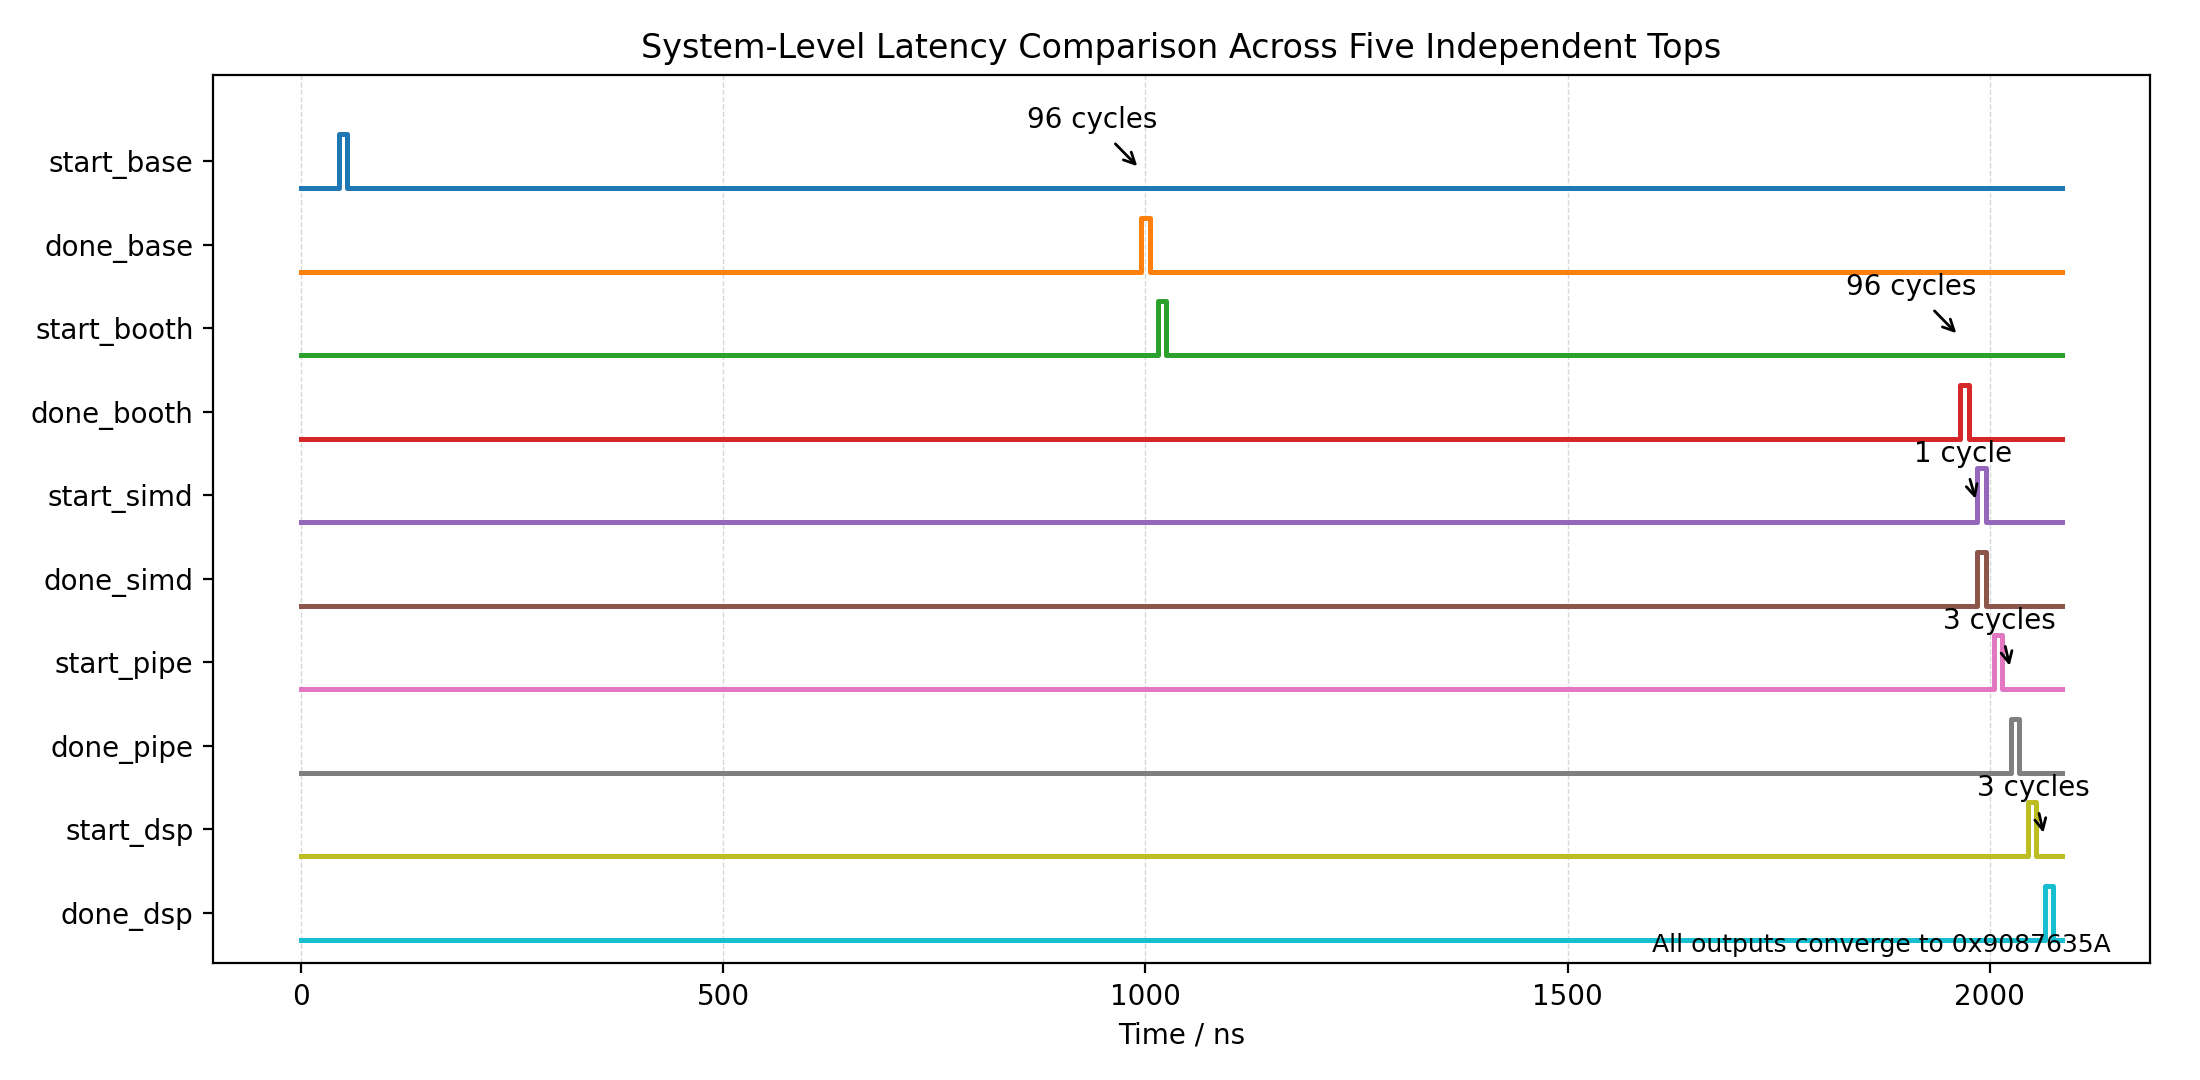
\includegraphics[width=\textwidth]{figures/wave_system_latency.png}
  \caption{系统级波形：串行顶层的 \texttt{start}/\texttt{done} 延迟}
  \label{fig:wave-system-base}
\end{figure}

\end{document}